% Generated from the editable Gate_4 sources by build_paper.py.
\documentclass[lineno,pdflatex,sn-nature]{sn-jnl}
\usepackage{graphicx,amsmath,amssymb,booktabs,xcolor}
\setcitestyle{super,comma,open={},close={}}
\renewcommand{\bibnumfmt}[1]{#1.}
\urlstyle{same}
\setlength{\emergencystretch}{2em}
\raggedbottom
\hypersetup{hidelinks,pdftitle={Bounding the rate loss of individual paired wireless uplink schedules},pdfauthor={Pooya Hejazi and Masoud Sabaei}}
\begin{document}
\title{Bounding the rate loss of individual paired wireless uplink schedules}
\author[1]{\fnm{Pooya} \sur{Hejazi}}
\author*[1]{\fnm{Masoud} \sur{Sabaei}}\email{sabaei@aut.ac.ir}
\affil[1]{\orgdiv{Department of Computer Engineering}, \orgname{Amirkabir University of Technology}, \orgaddress{\city{Tehran}, \country{Iran}}}
\abstract{Certifying coupled discrete--continuous decisions requires bounding every competing action on the same noisy instance. We study paired uplinks with two single-antenna users per tone and separate linear filters without successive interference cancellation, combining power-interval bounds, a checkable matching certificate and error calibration along the deployed filters. Outward-rounded arithmetic separates an achievable rate from a global ceiling and decomposes their difference into four nonnegative terms. Across 512 topologies at each of 32 and 64 users, deterministic search gives median gaps of 0.061 and 0.067 bit/s/Hz in 18 and 80 ms, retaining median rates above 99.5\% of the best certified ceiling. Message-passing price proposals did not establish a benefit over compute-matched deterministic controls. On successive recorded array pilots, phase-invariant calibration raises conservative floors to 24--28\% of later rates, although local-clock residual coverage remains below nominal.}
\maketitle



Coupled discrete--continuous allocation poses two computational tasks: finding a feasible decision and certifying its distance from the best alternative on the same instance. Paired uplinks expose this distinction under noise and a deadline: partner selection, tone assignment and transmit powers jointly determine interference at the receive array. Pilot reuse limits coherent processing~\cite{marzetta}; distributed access points, minimum mean-square error (MMSE) reception and user-specific antenna groups improve separation~\cite{ngo,bjornson,demir,buzzi}. Ergodic bounds and optimized precoders characterize attainable rates~\cite{caire,wang}, but a scheduler needs a certificate for its particular observation.

Uplink experiments established the throughput benefit of channel-adaptive transmission~\cite{haustein}. Matching identifies compatible users in an equal-energy window~\cite{viterbo}, and exact discrete search benchmarks LTE pairing with prescribed powers~\cite{fan}. Ruder and colleagues use Blossom pairing and small-system enumeration for joint grouping and frequency allocation~\cite{ruder2013}, later comparing predicted CSI with perfect-CSI search while assuming perfect CSI for payload detection~\cite{ruder2014}. Prasad and colleagues give approximation guarantees and instance-dependent upper benchmarks without knapsack constraints~\cite{prasad}. Water-filling solves a large-system limit; alternating transceiver updates and fractional programming address continuous powers and discrete assignments~\cite{viswanath,shi,shenfpone,shenfptwo}.

Learning can accelerate the search. Neural power control, graph networks and learned clustering exploit interference structure and user symmetry~\cite{sun,shen,hejazicluster,ahmadi2026}. Hardware Ising optimization schedules independent sets~\cite{hamakawa2026}, while throughput feedback adapts discrete beam and power settings~\cite{kashimata2026}. These approaches motivate a separate question: what gain remains when the controller stops? Predicted prices can initialize exact bipartite solvers or yield constraint-programming bounds~\cite{dinitz,bessa}. We instead verify proposed prices against every candidate pair and tone.

Here we construct an integer-checkable odd-set matching relaxation~\cite{edmonds,kuhn} with an exact four-term gap identity, implement outward-rounded binary64 and quarter-tick verification, and calibrate uncertainty along deployed decision operators. Full-channel uncertainty protects the competing oracle, while projected errors tighten the achievable floor of stored filters. Standardized channels, ray traces and recorded pilots test scalability and numerical reproducibility~\cite{tr,sionna,deepmimo,zafari,renew,shepard}. Supplementary Note~1 and Supplementary Table~1 compare ten related studies.

\section*{Results}

\subsection*{An interval for each uplink decision}

We consider full-service paired uplinks with two single-antenna users per tone, one tone per pair and \(K=2S\). Powers are bounded, and separate linear receive filters treat the partner as interference without successive interference cancellation. A decision specifies the pairs, their distinct tones, powers and stored filters. The lower endpoint \(L\) bounds the sum rate achieved by that particular action. To construct the ceiling \(U\), we allow competing schedules to choose different partners, tones, powers and receive filters. The interval contains both the achieved rate and the optimum, conditionally on the calibrated error events for uncertain channels. The largest improvement a competitor could deliver is therefore bounded by \(G=(U-L)/(S\ln 2)\) in bit/s/Hz, where \(U\) and \(L\) are aggregate nats and \(S\) is the number of occupied tones.


To obtain the ceiling, we price total power, bound the rate of every pair on every tone throughout its feasible power rectangle and temporarily let each pair use its favourite priced tone. A maximum-weight perfect matching remains, certified by prices for vertices and certain odd sets. The checker tests each edge inequality and compares the matching and dual objectives for equality. Related branch-and-price and mixed-monotonic algorithms also exploit bounds to organize difficult searches~\cite{barnhart,matthiesen}. A valid interval is available at any stage for which a full-domain upper bound and a feasible lower rate have both been checked. Assigning distinct tones, feasible powers and receive filters to the selected pairs produces such a lower rate. 


The same price table explains the width of the interval (Fig.~\ref{fig:arch}). The first term is the slack in the upper certificate after pricing the selected partners. With an exact matching witness it equals the weight lost by choosing those partners over the price-optimal matching. The next two give the cost of assigning distinct tones to those partners and the price of unused power. The fourth measures the difference between the local power bound and the achieved-rate floor. All four are nonnegative and sum exactly to \(U-L\). A zero unused-power term can therefore coexist with appreciable slack from pairing, tone assignment or the rate enclosure. If an alternative schedule improves the lower endpoint, its tone penalty follows its own pairs. The preferred pairs used to compute the upper bound can have a different penalty. Supplementary Note~2 gives the complete derivations and proofs.




\subsection*{Competition for tones survives optimal pricing}

With divisible spectrum, time sharing can close a duality gap or support convexification of an interference problem~\cite{yului,zhaopottie}. A labelled tone in our uplink is indivisible. Complexity results for three-dimensional matching, interference alignment and non-orthogonal multiple access illustrate the difficulty of related assignments under different receiver models~\cite{dyer,razaviyayn,salaun}. Here four users suffice to show exactly a limit of tone pricing. At unit power and noise, take channel vectors \((1,0),(0,1),(3/5,4/5),(-4/5,3/5)\) on the first tone and interchange the middle two on the second. Each tone has two disjoint pairs whose channel vectors are orthogonal, but can serve only one of those pairs. A pair with squared normalized channel overlap \(r\) earns \(2\ln(2-r/2)\). Of the six labelled schedules, four have a product of the two log arguments of \(91/25\) and two have \(1764/625\), so the best feasible rate is \(2\ln(91/25)\). Raising the price of either tone favours the orthogonal matching on the other. Even the best prices leave a ceiling of \(4\ln2\), exactly \(2\ln(100/91)\) aggregate nats above the feasible optimum (Fig.~\ref{fig:con}a,b).


For a given priced table, let \(R_\beta\) be the relaxed upper score, \(D\) the best score with all tone labels enforced, and \(A_\beta\) the score when the relaxed matching is assigned distinct tones. The price-selected pairs give a computable bound \(\Delta_{\mathrm{conflict}}=R_\beta-A_\beta\) on the exact relaxation loss \(R_\beta-D\). An alternative bound \(S\,d(\beta)\) uses the largest range of scores across all candidate pairs. We solved the labelled integer table exactly by dynamic programming on 512 simulated 16-user topologies at 10 dB. The posterior conflict statistic tracked the exact relaxation loss (Spearman \(\rho=0.665\), 95\% bootstrap interval 0.601 to 0.723). The all-edge range had virtually zero association (\(\rho=-0.005\), interval \(-0.093\) to \(0.080\), Fig.~\ref{fig:con}c,d). Pairs that never enter a competitive matching can dominate the range. Supplementary Fig.~1 shows the comparison within each profile.


Across 128 channels and nine selectivity levels, price-selected conflict never exceeded half the interval of a fixed sequential equal-power action: its largest ratio was 0.377. That action's own tone term exceeded half its gap in 980 of 1,152 cases. In optimized native decisions, mean tone terms were 0.0412 of a 0.0652-bit/s/Hz mean gap at 32 users and 0.0587 of 0.0722 at 64 users (Supplementary Fig.~2). Both matchings must therefore be identified. Separately, two-user rational stationary-point enclosures resolved continuous optima within \(5.2\times10^{-15}\) bit/s/Hz; bounded enumeration at four to eight users remained above \(10^{-6}\). These continuous references differ from exact integer-table comparisons.




\subsection*{Channel uncertainty enters through the receiver}
Error perpendicular to a deployed combiner leaves its output unchanged, whereas an oracle can rotate its filter. Channel-estimation bounds~\cite{hejazipilot} and conformal uncertainty sets under exchangeability~\cite{lei,johnstone} motivate separate information for these two receivers. We retain a full-channel ceiling \(U_F\), comparing a vector-ball floor \(L_F\) with a projected floor \(L_P\) for the same powers and filters. On their joint coverage event, the larger floor remains valid under the unchanged oracle ceiling (Theorems 3 and 4).

An orthogonal benchmark isolates the effect of pilot precision. With 16 receive dimensions, 32 users and unit powers, each user has a nominal channel of squared norm 160 that is orthogonal to its assigned partner's channel on the selected tone. Each channel has independent proper complex Gaussian error with variance \(1/32\) per complex component. Integrating the order statistics of the calibration-block maxima gives a mean oracle ceiling of 15.128 bit/s/Hz. Replacing the vector-ball floor with the projected floor cuts the expected gap from 3.1537 to 1.3353 bit/s/Hz, a tightening of 1.818 bit/s/Hz (Fig.~\ref{fig:unc}a). Supplementary Note~3 and Supplementary Table~2 give the order-statistic integrals and outward enclosures under two SNR conventions. Even with zero nominal cross projection, an error radius of about 0.50 admits interference power of \(0.50^2=0.25\) above unit noise. Together with the desired-amplitude reduction, this lowers the per-tone rate floor by 0.87 bit/s/Hz at squared nominal amplitude 160.


We compared fixed pilot energy with energy proportional to signal-to-noise ratio (SNR) on held-out clustered delay line C (CDL-C) and four-site urban macro (UMa) channels. Figure~\ref{fig:unc}d counts a usable decision when the projected lower rate is positive (\(L_P>0\)), the gap \((U_F-L_P)/(S\ln2)\) is at most 0.50 bit/s/Hz, retention \(L_P/U_F\) is at least 0.95 and the computation finishes within 1 s. At 32 users and 10 dB, all 128 CDL-C topologies met these four conditions at both pilot energies. On UMa the count rose from 83 to 127 of 128. Median gaps fell from 0.402 to 0.167 bit/s/Hz on CDL-C and from 0.466 to 0.274 on UMa (Fig.~\ref{fig:unc}b,c). Testing both error events against the simulated channel gave 120 of 128 joint coverage hits on CDL-C and 127 of 128 on UMa for each energy policy. The exact two-sided 95\% Clopper--Pearson intervals were 88.06--97.26\% and 95.72--99.98\%, respectively. The lower-tailed binomial test against 0.95 did not reject for either family at 10 dB. With only 16 calibration blocks, the required rank instead gives an infinite radius and no informative rate guarantee.




\subsection*{Rate guarantees for 32 and 64 users}

The primary comparison required a gap of at most 0.15 bit/s/Hz and a decision time of at most 250 ms for 32 users or 1,000 ms for 64. The same 512 independent 64-user channel realizations supplied nested 16-, 32- and 64-user subsets; the sizes are paired observations, not independent cohorts. This gave equal weight to the three single-site clustered delay line profiles (CDL-A, CDL-B and CDL-C) and the four-site urban macro profile. The deterministic scheduler, which updates the prices of congested tones and exchanges partners across feasible matchings, succeeded on 506 of 512 (98.83\%) and 504 of 512 (98.44\%) topologies. The exact one-sided 97.5\% Clopper--Pearson lower limits were 97.47\% and 96.94\%; the within-profile bootstrap limits fixed before test evaluation were 97.85\% and 97.27\%, respectively. Median gaps were 0.0613 and 0.0666 bit/s/Hz. Certificate-inclusive median times were 17.9 and 79.6 ms, and the 95th percentiles of individual calls were 33.2 and 140.3 ms (Fig.~\ref{fig:scale}a--c). All eight unsuccessful 64-user decisions arrived on time but exceeded the gap threshold, and all came from UMa. Supplementary Note~4, Tables~3--5 and Figs.~3 and 4 detail these comparisons.


Simple matching already delivered high rates in these 16-antenna simulations. Zero-price matching, matching with power refinement and the subgradient baseline shared the same initial matching and power-refinement trajectory, giving identical lower endpoints on every topology. Their median lower rates at 16, 32 and 64 users were 15.1362, 15.2885 and 15.4007 bit/s/Hz, retaining 99.45\%, 99.32\% and 99.39\% of the best ceiling selected within each topology; sequential equal-power pairing retained 93.43\%, 92.32\% and 91.78\%. Deterministic search raised the median lower rate by only 0.0566, 0.0427 and 0.0294 bit/s/Hz (0.37\%, 0.28\% and 0.19\%). Its larger benefit was a tighter ceiling: at 32 users, median gaps fell from 0.5133 for zero-price matching and 2.1464 for matching with power refinement to 0.0613 bit/s/Hz; at 64 users they fell from 0.4882 and 2.1219 to 0.0666. Deterministic search retained 99.636\% and 99.587\% of the best ceiling at these two sizes (Fig.~\ref{fig:phase}a; Supplementary Table~6).


A three-layer message-passing network supplied additional starting prices alongside the complete deterministic branch. It recovered all six failures at 32 users and five of eight at 64, retaining previous successes. Median gaps became 0.0549 and 0.0645 bit/s/Hz, with median times of 42.6 and 177.2 ms, respectively. Gains of 1.17 and 0.98 percentage points fell below the ten-point learning target; exact paired comparisons with the original baseline gave \(P=0.03125\) and \(P=0.0625\). Used alone, the network passed on 303 of 512 and 340 of 512 topologies.

We reran all 512 topologies per size with three repeats and rotating order. Absolute times differed between the primary campaign and these exploratory reruns. Three extra deterministic price iterations gave 507 of 512 and 505 of 512 passes, with median gaps of 0.05942 and 0.06612 bit/s/Hz. Learned warm start gave 512 of 512 and 509 of 512. Against this iteration-matched control, learned-only successes numbered five and four, with none favouring the control: exact two-sided McNemar \(P=0.0625\) and \(P=0.125\). Relative to the rerun baseline, the added median times were 2.5850 and 6.7841 ms for extra iterations, versus 22.7841 and 95.4903 ms for learning. The learned median lower-rate gains over deterministic search were 0.00440 and 0.00110 bit/s/Hz, and the two methods had the same 64-user median ceiling, 15.4897 bit/s/Hz.


A separate timing-only pilot fixed a larger deterministic budget of 38 and 63 price iterations. On the full paired cohort, its median times were 38.39 and 176.35 ms, slightly exceeding the contemporaneous learned times of 35.59 and 164.01 ms. It passed on 507 of 512 and 505 of 512 topologies, with median gaps of 0.05783 and 0.06318 bit/s/Hz. The learned counts remained 512 of 512 and 509 of 512, again with five and four learned-only successes and \(P=0.0625\) and \(0.125\) (Fig.~\ref{fig:scale}d; Supplementary Table~7). Neither control establishes a learning advantage at the 0.05 level; the larger deterministic budget gives the smaller 64-user median gap.


Component swaps also separated proposals from verification. On 32-user UMa, changing box order preserved a 0.074-bit/s/Hz median gap, whereas learned anchors, prices or actions widened it (Supplementary Table~4). Constructing and bounding the pair--tone table dominated 64-user deterministic time (median 50.9 ms).

For two-user analytic channels, the exact continuous reference divides a mean gap of 0.23808 bit/s/Hz into 0.23467 of ceiling slack and 0.00340 of real action loss. The ceiling slack alone exceeds the 0.15 criterion. Its median is much smaller, 0.00221 bit/s/Hz (IQR 0.00006--0.13947), showing the influence of difficult channels. At four, six and eight users, mean ceiling slack is at least 0.12743, 0.05487 and 0.03387 bit/s/Hz. The median reference widths are \(5.85\times10^{-5}\), \(7.34\times10^{-5}\) and \(1.50\times10^{-4}\), but maxima of 0.514, 0.854 and 0.929 leave the mean slack and loss split unresolved. Figure~\ref{fig:phase}b and Supplementary Table~8 therefore report means, medians and endpoint quartiles. The separate 16-user native-channel row measures slack above, and shortfall below, the exact integer upper-table optimum. That table optimum bounds the physical optimum; its shortfall is not a measured physical rate loss.


Propagation geometry also changes tightness. Across 64 guarded tiles per scene at 10 dB, median gaps at 32 and 64 users were 1.120 and 1.096 bit/s/Hz on the 60-GHz O1 street versus 0.102 and 0.095 on the 3.5-GHz ASU campus. Median squared channel overlaps were 0.9936 on O1 versus 0.4649 and 0.4578 on ASU, with Gram effective ranks near one versus 2.6 (Supplementary Note~5, Supplementary Table~9 and Supplementary Fig.~5). O1's nearly parallel vectors limit spatial separation. Experiments with transmitting and receiving apertures show how geometry changes focusing and resolvable modes~\cite{kludze2026,shenoam2026}; our independently transmitting users also occupy different scene footprints, so carrier frequency alone cannot explain the contrast.

At 32 users, median local-bound contribution \(T_4\) was 1.1133 on O1 versus 0.0074 on ASU. Refining 32, 128, 512 or all 7,936 pair--tone entries into 16 children changed no upper-table entry. The top-32 shortlist contained a median of two scheduled entries. Refining all 16 scheduled entries, with action and prices fixed, gave median \(T_4=1.113253\) and \(G=1.119582\) bit/s/Hz at the baseline depth of 16 children. At 64 and 256 children, median \(T_4\) fell to 1.080005 and 0.867040, respectively, whereas median \(G\) fell only to 1.118334 and 1.117494 bit/s/Hz. Unrefined alternatives keep the ceiling loose (Supplementary Table~10).

Continuous references on all 64 nested two- and four-user O1 problems give mean ceiling slacks of 1.03877 and 0.90425 bit/s/Hz versus mean action losses of 0.13522 and 0.15193 bit/s/Hz, respectively. Polynomial-root enclosures and exhaustive labelled references, the latter resolved to \(10^{-6}\) bit/s/Hz, identify ceiling conservatism as the larger small-system contribution. They do not establish the exact 32-user decomposition.



\subsection*{The cost of additional pilots}
We compared power-refined zero-price matching with learned warm start on the same least-squares estimate, charging both for routine pilots. Without additional calibration pilots, learned warm start had a certified positive net advantage on 0 of 128 fixed-energy CDL-C, 28 of 128 scaled-energy CDL-C, 12 of 128 fixed UMa and 111 of 128 scaled UMa topologies. Sixteen extra pilot blocks exhausted scaled UMa's one-block budget; amortizing that charge across 256 and 1,024 blocks yielded advantages on 10 and 74 of 128 cases, respectively (Fig.~\ref{fig:phase}c,d). This accounting assumes stationary per-block rates (Supplementary Note~5, Supplementary Table~11 and Supplementary Fig.~6).



\subsection*{Receiver performance on successive recorded pilots}
Six-user Rice RENEW recordings supply early channels and later pilot observations~\cite{zafari,renew}. After noise whitening, the shared-reference-clock (HUB) capture achieved \(G\leq0.10\) bit/s/Hz within 250 ms on 1,867 of 1,873 post-calibration frames; the local-clock (LO) capture passed on 1,037 of 1,873. Median times were 2.75 and 2.71 ms, respectively (Fig.~\ref{fig:hw}a; Supplementary Note~6, Supplementary Table~12 and Supplementary Fig.~7). Denominators include detection failures.

Holding the action and filters fixed, every eligible later-pilot rate fell below its early floor: median differences were \(-2.501\) and \(-4.873\) bit/s/Hz on HUB and LO, respectively (Fig.~\ref{fig:hw}b). The disjoint long-training-sequence windows begin 16~\(\mu\)s apart. Filter design and evaluation on the same noisy early pilot create in-sample optimism; this replay cannot separate noise, synchronization and evolution. Dedicated experiments can isolate synchronization and reciprocity offsets~\cite{rogalin,vieira,ganesan}, including clock feedback switched over optical fronthaul~\cite{zhangsync2026}. Here each clock mode has only one independently documented acquisition layout.

We asked whether removing phase sensitivity could make the recorded-pilot floors more informative. Raw complex-difference calibration used the first 256 eligible frames and tested 1,614 HUB and 1,513 LO frames. Median full-vector floors \(L_F\) were 3.050 and 0.978 bit/s/Hz, versus projected floors \(L_P\) of 3.754 and 1.292. The later-rate medians were 21.937 and 18.927 bit/s/Hz; the median paired floor fractions were only 17.15\% and 6.76\%. Vector-to-projected radius ratios were 1.153 and 1.145, compared with 2.144 in the Gaussian benchmark. Raw interval widths were 23.075 and 26.830 bit/s/Hz. All floors held, but LO achieved only 70.26\% joint residual coverage against a nominal 95\%: calibration failed to reach its target, and the rate floors held through slack.


Median absolute phase rotations were 0.0419 rad on HUB (IQR 0.0200--0.0712) and 0.2599 rad on LO (0.2331--0.2863), equivalent to 0.417 and 2.586 kHz, respectively, over 16~\(\mu\)s if entirely attributed to frequency offset. These diagnostics do not identify oscillator drift. Fixed-filter independent pilot noise predicts a projected maximum near 2.45 whitened units (97.5\% union bound 3.51), far below raw projected radii of 87.36 and 165.26 on HUB and LO.

Fixed-combiner SINR depends on projection magnitudes, permitting phase-invariant calibration. With the same split and rank 251, projection-magnitude residuals reduced projected radii to 59.52 and 70.30; phase-aligned vector radii were 81.10 and 111.72. Median projected floors rose to 6.028 and 4.564 bit/s/Hz (27.51\% and 24.46\% of paired later rates), with vector floors of 4.155 and 2.514. Median widths narrowed to 20.421 and 22.246 bit/s/Hz. Floor and interval coverage remained 100\%, while joint residual coverage was 98.08\% on HUB and 75.74\% on LO (Fig.~\ref{fig:hw}c,d; Supplementary Table~13). Phase invariance improves the useful floor, but does not restore nominal calibration on LO. Exhaustive fixed-equal-power enumeration of all 90 early-input schedules remained within median ceiling excesses of \(3.33\times10^{-5}\) and \(6.86\times10^{-5}\) bit/s/Hz. Mean per-entry difference powers were 18.40 on HUB and 121.62 on LO, falling after phase alignment to 12.25 and 43.95, respectively, still above the independent-noise prediction of two. Against mean early powers of 1,256.87 and 1,074.46, these aligned residuals are \(-20.11\) and \(-13.88\) dB: signal-dependent error or underestimated pilot-period noise could explain the excess, but these stored pairs cannot distinguish them (Supplementary Table~13).


The separate Argos spatial-overlap measurements are reported in Supplementary Table~14 and Supplementary Fig.~8. They describe user separation in a fixed array, complementing experiments that change array connectivity to measure signal gain~\cite{ni2026}. They do not measure a scheduled paired-payload transmission.



\section*{Discussion}

The central computational contribution is a checkable ceiling for one decision. In these well-conditioned arrays, simple matching already retains over 99.3\% of the best ceiling; tightening certification produces modest additional throughput. The derivation covers full-service paired uplinks. Different multiplexing orders, multiple tones per user, successive interference cancellation or queue or fairness weights require new bounds.

Separating ceiling slack \(U-V\) from action loss \(V-L\) matters whenever global optimization is stopped early. The four-term identity localizes computational slack, but does not itself measure physical suboptimality. Exact small-system references reveal predominantly ceiling slack and nonzero action loss; wide reference tails and unrefined alternatives limit extrapolation to larger problems. 

The iteration- and median-time-budget controls similarly separate neural proposals from additional computation. Their \(P=0.0625\) and \(P=0.125\) comparisons do not establish a learning advantage; at 64 users additional deterministic search gives the smaller median gap. Remaining uncertainty can guide further computation, but the primary 18--80-ms medians suit slowly changing channels or upper-layer allocation. Millisecond control requires a separately timed implementation with reduced work or acceleration.

Calibrating along deployed decision operators can tighten uncertainty bounds without weakening a valid oracle ceiling. Recorded-pilot floors improve to 24--28\% of later rates, yet LO residual coverage remains below nominal. The mathematical construction does not repair distribution shift or temporal dependence. If quiet-slot variance understates active-period noise and distortion, hardware rates are optimistic and gaps and pass fractions require recalculation with an appropriate noise model. Extending it to live control requires transmitting the selected actions, retaining their filters and measuring decoded payload over the scheduling delay, with independent acquisitions to establish reproducibility.
\section*{Online Methods}
\subsection*{Channel, feasible decisions and opportunity loss}
A receiver with \(N\) jointly processed antenna streams serves \(K=2S\) users on \(S\) labelled, orthogonal tones of equal bandwidth. Each user transmits one independent unit-variance Gaussian symbol on its assigned tone. For the two users \(i,j\) on tone \(s\), the whitened observation is \(y_s=\sqrt{p_i}h_{is}x_i+\sqrt{p_j}h_{js}x_j+n_s\), where the complex noise has covariance \(I_N\). In simulation, powers satisfy \(0.05\leq p_i\leq0.20\) W and \(\sum_i p_i\leq P=0.10K\) W. The Rice replay instead uses digital receiver units. The oracle serves every user once, optimizes within these power limits and uses a separate linear combiner for each user, treating its partner as interference.

For nonzero \(h_{is}\), Cauchy--Schwarz in the interference-plus-noise inner product gives the optimal combiner direction \((I_N+p_j h_{js}h_{js}^{H})^{-1}h_{is}\). Let \(x=p_i\|h_{is}\|^2\) and \(y=p_j\|h_{js}\|^2\). The squared normalized overlap \(r=|h_{is}^{H}h_{js}|^2/(\|h_{is}\|^2\|h_{js}\|^2)\) is set to zero if either channel vanishes. The received signal-to-interference-plus-noise ratios and pair rate in nats are
\begin{equation}
\begin{aligned}
\gamma_i &= x\left(1-\frac{r y}{1+y}\right), &
\gamma_j &= y\left(1-\frac{r x}{1+x}\right),\\
q_{e,s} &= \ln(1+\gamma_i)+\ln(1+\gamma_j), & e&=\{i,j\}.
\end{aligned}
\label{eq:sinr}
\end{equation}
The oracle rate \(V(h)\) maximizes the sum of pair rates over a finite set of schedules and a compact set of powers. Evaluating the stored filters at the implemented powers gives the Gaussian-input mutual information \({R_{\mathrm{fix}}}(h)\), assuming that the decoder knows the effective scalar complex gain \(v_i^Hh_{is}\) after combining, even when those filters are suboptimal. These are gross occupied-band rates; pilot overhead is deducted only in the stationary net-rate calculation. Valid endpoints therefore imply the instance-wise bound \((V(h)-{R_{\mathrm{fix}}}(h))/(S\ln 2)\leq G\).

\subsection*{Theorem 1: a full-domain matching certificate}
The power bound, matching relaxation, vertex-price repair and signed rounding are given as self-contained arguments. Complete derivations appear in Supplementary Note~2.

A power price \(\lambda\geq0\) lets us evaluate each pair separately while accounting for the total power budget. Assume \(0<p_-\leq p_+\) and \(P\geq Kp_-\). For a nonempty channel set \(\mathcal H\), let \(\mathcal Q=\mathcal H\times[p_-,p_+]^2\) contain the candidate channels and both users' feasible powers. Use \(H_{e,s}\) for the upper score of pair \(e\) on tone \(s\), and \(D(H)\) for the largest sum of table entries over feasible labelled schedules. Given tone prices \(\beta_s\in\mathbb R\), set \(w_e=\max_s(H_{e,s}-\beta_s)\) and let \(M(w)\) denote the maximum weight of a perfect user matching. For scores satisfying the first line below, the second line bounds every \(h\in\mathcal H\):
\begin{equation}
\begin{aligned}
 H_{e,s} &\geq \sup_{(h',a,b)\in\mathcal Q}
       \bigl\{q_{e,s}(a,b;h')-\lambda(a+b)\bigr\},\\[2pt]
 V(h)&\leq\lambda P+D(H)\leq\lambda P+\sum_{s=1}^{S}\beta_s+M(w).
\end{aligned}
\label{eq:upper}
\end{equation}
For the first rate inequality in equation~(\ref{eq:upper}), summing the pair bounds restores a power charge of at most \(\lambda P\). For the second rate inequality, each feasible schedule uses each tone once. Subtracting and restoring its tone prices leaves the score unchanged, and replacing each adjusted score by its maximum over tones gives an upper bound for the matching.

The checker verifies this last maximization using free vertex potentials \(\alpha_i\) and nonnegative prices \(z_B\) on a family \(\mathcal B\) of odd vertex sets~\cite{edmonds}. Write \(\mathcal B_e=\{B\in\mathcal B:e\subseteq B\}\). For every edge \(e=\{i,j\}\), the checker requires
\[
 \alpha_i+\alpha_j+\sum_{B\in\mathcal B_e}z_B\ \geq\ w_e .
\]
A perfect matching uses each vertex once and contains at most \(\lfloor |B|/2\rfloor\) edges inside \(B\). Summing the inequalities thus bounds its weight by \(\sum_i\alpha_i+\sum_{B\in\mathcal B}\lfloor |B|/2\rfloor z_B\). Equality with the proposed matching certifies optimality. When this witness is unavailable, any vertex prices give a bound after setting \(\beta'_s=\max_{e=\{i,j\}}(H_{e,s}-\alpha_i-\alpha_j)\). Summing over a feasible schedule then gives \(U=\lambda P+\sum_i\alpha_i+\sum_s\beta'_s\). Both vertex and tone prices may have either sign.

\subsection*{Theorem 2: label conflict and four-term accounting}
Let \(m_\beta\) attain \(M(w)\), \(R_\beta=\sum_s\beta_s+M(w)\), and \(A_\beta\) be the highest score of \(m_\beta\) when its pairs must occupy distinct tones, computed by bipartite assignment~\cite{kuhn}. Let \(d(\beta)=\max_e\{\max_s(H_{e,s}-\beta_s)-\min_s(H_{e,s}-\beta_s)\}\). Since \(A_\beta\) is feasible and \(R_\beta\) is an upper bound,
\begin{equation}
\begin{aligned}
0 &\le R_\beta-D(H)\le\Delta_{\mathrm{conflict}}=R_\beta-A_\beta,\\
\Delta_{\mathrm{conflict}} &=\sum_{e\in m_\beta}\bigl(w_e-H_{e,s(e)}+\beta_{s(e)}\bigr)
       \le S\,d(\beta).
\end{aligned}
\label{eq:conflict}
\end{equation}
The last inequality follows edge by edge. If \(H_{es}=a_e+b_s\), choosing \(\beta_s=b_s\) makes every edge range zero. Thus distinct tone labels cost nothing on a separable table, although the continuous-power enclosure can still contribute slack. In the four-user example, the two orthogonal disjoint matchings imply lower bounds \(4\ln2\pm(\beta_2-\beta_1)\) on \(R_\beta\). No edge can earn more than \(2\ln2\), so equal prices attain their common lower bound. Exhaustive evaluation of the six actual assignments then gives the stated positive discrepancy.

To decompose the interval for the delivered action, take the \emph{implemented} matching \(m\), its bijection \(s(e)\) and lower pair rates \(l_e\), all evaluated on the selected compatible table. For \(e=\{i,j\}\), write \(p_e=p_i+p_j\) and \(L=\sum_{e\in m}l_e\). Each \(l_e\) bounds the rate of the stored filters at the implemented powers on the channel event under consideration. For this decomposition the upper witness must satisfy \(U\geq\lambda P+\sum_s\beta_s+\sum_{e\in m}w_e\). The four terms are
\begin{equation}
\begin{aligned}
 T_1 &= U-\lambda P-\sum_s\beta_s-\sum_{e\in m}w_e,\\
 T_2 &= \sum_{e\in m}\bigl(w_e-H_{e,s(e)}+\beta_{s(e)}\bigr),\\
 T_3 &= \lambda\Bigl(P-\sum_i p_i\Bigr),\\
 T_4 &= \sum_{e\in m}\bigl(H_{e,s(e)}+\lambda p_e-l_e\bigr).
\end{aligned}
\label{eq:decomposition}
\end{equation}
The four terms are nonnegative by the upper witness, the edge maxima, power feasibility and the enclosure at the implemented powers, respectively. Summing them cancels the internal prices and scores, giving \(U-L=\sum_{j=1}^4T_j\) exactly. The assignment defining \(A_\beta\) belongs to the price-selected matching \(m_\beta\). The delivered schedule can use another matching from the candidate pool, in which case its \(T_2\) measures the label penalty for that action. The fourth term combines continuous-power enclosure slack, achieved-action suboptimality and downward rate rounding.

\subsection*{Theorems 3 and 4: achieved rates under calibrated error}
A fixed pilot-to-action map produces a feasible schedule, powers and nonzero filters. The same action is used for both lower endpoints. Write \(d_i\) for a filter normalized to unit length and \(s=s(i),j=j(i)\) for its tone and partner. Given a channel centre \(\hat h\) and directional radii \(b_{ik}\), define
\[
 \ell_i(b)=\frac{p_i\left[|d_i^H\hat h_{is}|-b_{ii}\right]_{+}^2}
                 {1+p_j(|d_i^H\hat h_{js}|+b_{ij})^2}.
\]
On the event \(|d_i^H(h_{ks}-\hat h_{ks})|\leq b_{ik}\) for the desired and interfering signal of every user, the sum of \(\ln(1+\ell_i)\) rounded down is \(L_P\leq{R_{\mathrm{fix}}}(h)\). The reverse triangle inequality bounds the desired amplitude from below, and the ordinary triangle inequality bounds the interfering amplitude from above. On the full-vector event \(\|h_{ks}-\hat h_{ks}\|\leq\epsilon_{ks}\), Cauchy--Schwarz gives the same formula with \(b_{ik}=\epsilon_{ks}\), yielding \(L_F\), and Theorem 1 gives \(U_F\). Hence, on their intersection (Theorem 3),
\[
       \max(L_F,L_P)\ \leq\ {R_{\mathrm{fix}}}(h)\ \leq\ V(h)\ \leq\ U_F .
\]
Whenever the queried directions leave an unobserved subspace, a channel component in that subspace can increase the oracle rate without changing those projections. The upper endpoint therefore requires the full-vector channel set.

For Theorem 4, condition on the fit and policy-selection data. The calibration blocks and the next test block must be exchangeable under this conditioning. The complete pilot-to-action map, including repairs and tie-breaking, and the positive scale functions \(\sigma_{ks},s_{ik}\) are fixed before calibration on data separate from the calibration blocks. Each block supplies two scores,
\[
\begin{aligned}
 T_F &= \max_{k,s}\frac{\|h_{ks}-\hat h_{ks}\|}{\sigma_{ks}},\\
 T_P &= \max_i\ \max_{k\in\mathcal K_i}
         \frac{|d_i^H(h_{k,s(i)}-\hat h_{k,s(i)})|}{s_{ik}},
 \qquad \mathcal K_i=\{i,j(i)\}.
\end{aligned}
\]
The scale functions may depend on a block's observed pilots through this frozen map. For \(a\in\{F,P\}\), take the \(\lceil(n+1)(1-\alpha_a)\rceil\)-th smallest calibration score, appending infinity at rank \(n+1\). Multiplying the two thresholds by their corresponding scales defines the vector and projection radii. For exchangeable calibration and test blocks, random tie-breaking makes the rank of the test score uniform. Including all ties can only increase coverage~\cite{lei}. Each event has marginal probability at least \(1-\alpha_a\), and the union bound gives joint coverage of at least \(1-\alpha_F-\alpha_P\) under arbitrary dependence among users, tones and scores. At \(n=256\), \(\alpha_F=\alpha_P=0.025\) gives rank 251 for each, and at \(n=16\) it gives rank 17. This coverage averages over calibration and test blocks before selection on the reported interval. An action selected after inspecting calibration residuals or the resulting radii requires separate calibration, or a block maximum covering every candidate action. If only a later noisy pilot is observed, transport to a true payload channel requires an additional error bound and its own error probability.

The analytic Gaussian experiment uses fixed unit powers, separately from the simulation power rails. Conditional on the specified channel centres, independent proper complex Gaussian errors have covariance \(\nu^2 I_{16}\). Set \(\nu^2=1/32\), \(A_0^2=160\), and let the two orthonormal directions have entries of magnitude \(1/4\). Each full score covers \(m=512\) independent links. Its squared normalized norm has gamma shape \(d=16\). Each projected score covers \(m=64\) independent scalar projections with \(d=1\). Their independence in this model follows from orthogonality and isotropic complex Gaussian errors. For \(F_d(x)=1-e^{-x}\sum_{j=0}^{d-1}x^j/j!\), the block cumulative distribution function (CDF) is \(F_d(q^2)^m\). At rank 251 among 256 blocks its CDF value has law \({\rm Beta}(251,6)\). For \(T\) with this law the physical radius has distribution \(\epsilon=\nu\sqrt{F_d^{-1}(T^{1/m})}\). For unit powers the per-tone upper and lower functions in bit/s/Hz are
\[
 u(x)=2\log_2(1+(A_0+x)^2),\qquad
 l(x)=2\log_2\!\left(1+\frac{\left[A_0-x\right]_{+}^2}{1+x^2}\right).
\]
We integrated \(u(\epsilon_F)-l(\epsilon_F)\) and \(u(\epsilon_F)-l(\epsilon_P)\) over the radius distributions. Two quadratures in different coordinates agreed within \(2\times10^{-8}\). A 144-fractional-bit rational enclosure, using monotone bin bounds and an explicit Erlang tail, bounded the gaps in \([3.151125,3.156294]\) and \([1.333129,1.337516]\) bit/s/Hz. The quadratures give 3.1537 and 1.3353 bit/s/Hz to four decimal places. The wider intervals enclose the expectations rigorously.

\subsection*{Building and checking the interval}
The input is a complex \(K\times N\times S\) array with uncertainties in whitened units. We round channel centres to a common dyadic grid with integer components bounded by \(2^{22}\). For \(N\leq256\), each real or imaginary Gram sum fits the exact integer range through \(2^{53}\). We enlarge the supplied vector radius by an outward bound \(\sqrt{2N}\,\delta/2\) on the Euclidean rounding displacement, where \(\delta\) is the grid spacing. For centres \(a,b\) and radii \(u,v\), the magnitude of their inner product is at least \(\left[|a^Hb|-\|a\|v-\|b\|u-uv\right]_{+}\). Dividing its square by the product of upper squared norms gives a lower bound on the squared normalized overlap when that product is positive. A zero product gives overlap zero. Bounding (\ref{eq:sinr}) with upper desired power and gain, lower interfering power and gain, and lower correlation encloses every realization in a power rectangle. We subtract the minimum power charge, and additionally take the better of that enclosure and a verified bound using tangents to the two individual concave log terms with a separately bounded correlation penalty.

Every pair and tone receives an upper bound on the entire two-user power rectangle before refinement begins. A change in price can reuse an unpriced enclosure. For each edge the two highest candidate tones enter a refinement shortlist. No more than \(\max(2,\lfloor K^2/32\rfloor)\) entries are fully divided into 16 rectangles. After all children cover a complete partition, the maximum child upper bound may tighten the parent. The stored bound is the minimum of that maximum and the parent bound. All other parents are retained. The priority score affects which entries tighten within the available time. The binary64 implementation uses nearest-even rounding with outward next-representable adjustments, gradual underflow and disabled fast-math reassociation. It range-reduces logarithms by powers of two, uses outward tabulation at \(1+j/256\) and a positive atanh series with a bounded remainder. Out-of-range or nonfinite data are rejected. The outward bounds certify the upper endpoint. Supplementary Note~7 and Supplementary Table~15 specify the numerical kernel and distinguish optional-leaf counts from total enclosure evaluations.

Each table entry is rounded \emph{up} to an integer multiple of \(2^{-40}\) nats before forming weights. The excess from rounding a schedule of \(S\) edges is less than \(S/2^{40}\) nats. A C++14 implementation using LEMON 1.3.1~\cite{lemon} exports a perfect matching, vertex prices and positive odd-set prices. An independent integer checker verifies the matching, every inequality and exact objective equality in the solver's quarter-tick potential units. The distinct-tone assignment and its potentials are also checked. A failed matching witness invokes the vertex-price repair described above. The stored powers are in units \(1/(20\cdot2^{20})\) W. Power projection enforces both rails and the total budget with integer arithmetic. The actual complex filter \(v_i\) is retained unnormalized. Directed dot products enclose both signal terms and the noise contribution \(\|v_i\|^2\) in its SINR denominator. Integer decomposition numerators, their common denominator, per-pair floors, selected leaves, actions, prices and input/table hashes identify precisely what was checked.

\subsection*{Small-instance continuous and discrete references}
We evaluated the labelled-table optimum by integer dynamic programming on the same rounded table used by the certificate. Exhaustive enumeration on smaller tables checked this discrete calculation. Continuous-power reference calculations used the stated power rails and total budget on 512 analytic channel blocks, with all labelled schedules enumerated at \(K=2,4,6,8\). An outward power-box search kept the best feasible lower bound and the largest remaining upper bound, with a budget of 192 subdivisions per instance and a target width of \(10^{-6}\) bit/s/Hz. The median remaining widths were \(5.8534\times10^{-5}\), \(7.3372\times10^{-5}\) and \(1.5043\times10^{-4}\) bit/s/Hz at \(K=4,6,8\), respectively. These medians are approximately three orders of magnitude below the 0.15-bit/s/Hz scheduling criterion. The reference brackets nevertheless have long tails, reaching 0.514, 0.854 and 0.929 bit/s/Hz, respectively. All 512 cases at each size remain wider than the finer target tolerance; conclusions use their enclosing intervals rather than treating their midpoints as exact optima.

For two users, a separate calculation resolves the continuous problem. With total power 0.20 W and positive channel gains, scaling both powers upward increases both signal-to-interference-plus-noise ratios until the sum constraint is tight. The feasible boundary is therefore \(p_2=0.20-p_1\), \(0.05\leq p_1\leq0.15\) W. Exact rational Gram coefficients reduce stationarity to a polynomial equation. We isolated its real roots in intervals of width at most \(2^{-75}\), included both boundary endpoints and evaluated outward logarithmic bounds at all candidates. All 512 resulting intervals met the \(10^{-6}\) bit/s/Hz target. This separate root calculation supplies the two-user continuous reference, whereas the integer dynamic program supplies the labelled optimum for a specified upper-bound table.

\subsection*{Price search, feasible schedules and learned proposals}
The deterministic route uses a price for power derived from the median single-user marginal rate and seven tone-price proposals through 32 users, six at 64. The first prices are zero. Subsequent anchors include centred mean scores and the tone potentials of a relaxation with two user slots per tone. To update the most promising price vector, we count excess favourite-tone requests from matched pairs and from individual user neighbourhoods. Centred assignment potentials receive weight 0.58 and the previous prices 0.42; the demand correction uses 0.75 pair and 0.25 neighbourhood weights, with a decreasing step starting at 0.05. These settings control how quickly the search tightens the interval. The same checker accepts each resulting bound.

We collect the sequential pairing, matchings from the successive prices and up to six promising disjoint edges per tone. Distinct-tone assignments, exchanges of tone labels, and exchanges of partners between two pairs generate feasible alternatives. For up to three promising schedules, we attempt four projected gradient updates. Each gradient is normalized by its largest absolute component, with a \(10^{-12}\) floor, and multiplied by \(0.05\) W and successive relative steps \(1,1/2,1/4,1/8\). Each proposal is projected onto the stored feasible powers and accepted if the nominal pair-rate sum does not decrease. The filters are then recomputed for those powers. The incumbent maximizes the checked lower bound across these candidates. We combine the smallest checked upper with the best feasible lower, evaluating the four terms on that upper's table and the final lower's action.

The learned proposer uses width 32 and three residual message-passing layers. Each pair--tone factor receives its current state, the pair and tone embeddings, and the sum and absolute difference of its two user embeddings. Means across tones and pairs update the corresponding nodes. Incident pair messages update each user. Heads propose pair--tone scores, powers, centred prices, a power price, box anchors and priorities. Training combines balanced positive/negative schedule loss, squared errors for powers, prices and anchors, and relative-priority losses. A centred optimal-assignment tone potential on the teacher's selected schedule supplies a price target. Three seeds (1729, 2718, 3141) each saw 4,096 blocks for 15 epochs with Adam (step \(10^{-3}\), size-homogeneous batches up to eight, gradient norm cap 3). Fit data comprised clustered-delay-line (CDL) profiles A, B and C and analytic channels at 8, 16 or 32 users. Four-site urban-macrocell (UMa) and 64-user examples were withheld from fitting. The mean validation fraction below gap thresholds 0.02, 0.05, 0.10 and 0.15 on 256 other blocks selected seed 1729. The learned warm start adds three price proposals to the entire deterministic branch. In the exploratory control, three more updates of the same deterministic rule replace those learned proposals; all methods use the same channels, three repeated calls and rotating order. The baseline rerun reproduced all 1,024 archived deterministic gaps. Equal counts of price iterations do not include equal neural inference or action-pool costs, so complete elapsed times are reported separately. A separate comparator uses one forward pass. Both learned routes retain full-domain verification. Supplementary Note~4 gives the layer equations, losses and solver pseudocode. In the combined route, learning adds price proposals to the deterministic table. Learned power prices, tangent anchors and leaf priorities affect the separate standalone comparator. On a Quadro RTX 4000 Max-Q, the synchronized standalone forward pass had 95th-percentile latencies of 15.65 ms at 32 users and 65.63 ms at 64 users.

\subsection*{Channels, uncertainty and measurement processing}
The native experiments used Sionna 2.2.0, with \texttt{spec\_version='19.2'} for CDL and UMa, selecting the 3GPP TR 38.901 version 19.2.0 parameter tables~\cite{tr,sionna}. At 3.5 GHz the three single-site profiles used a 16-element array and 100-ns delay spread. UMa used four 4-element arrays, at height 25 m on the corners of a 500-m square, with outdoor users at 1.5 m sampled uniformly within the central 420-m square. Path loss and shadowing were enabled. Sixty-four bins at 312.5 kHz spacing spanned 20 MHz. Nested user counts and evenly spaced labelled bins came from the same realization. A common block scale set the median per-antenna signal-to-noise ratio (SNR) at 0.1 W to the target value before cropping; this is a comparison of normalized channels. The analytic controls used nearly parallel users, frequency-flat channels, frequency-selective channels and an orthogonal benchmark. In the orthogonal benchmark, the construction enforces orthogonality between the two partners assigned to each tone in the reference schedule. The two ray-traced scenes used base station 1, the O1 60-GHz and ASU 3.5-GHz source files, and 64 disjoint guarded tiles each, avoiding pilot tiles and their immediate neighbours. We considered \(-5,0,10,20\) dB and 16, 32 or 64 users in the wider sensitivity grid (13,824 cells). The two primary endpoints used the native 10-dB channels at 32 and 64 users. Relative to the operating sum rates of each regime, these absolute gap criteria correspond to roughly 1\% of the certified ceiling on known channels (0.15 bit/s/Hz), 2.6--3.3\% of the median ceiling under noisy pilots at 10 dB (0.50 bit/s/Hz), and 0.41--0.42\% of the median early lower rate on the six-user hardware captures (0.10 bit/s/Hz).

To interpret differences between the two ray-traced scenes, we examined the stored user vectors and the base-station ray records for the same held-out users. For each tile we averaged \(r\) over distinct user pairs and tones. On each tone we also formed the Gram matrix of unit-norm user vectors and computed its effective rank \(\exp(-\sum_j t_j\ln t_j)\), where \(t_j\) are its eigenvalues divided by their sum and \(0\ln0=0\). We averaged ranks over tones before summarizing tiles. As a separate measure of sensitivity to partner choice, we held both powers at 0.10 W and used equation~(\ref{eq:sinr}) to evaluate each user's rate with every possible partner. We averaged the difference between the 90th and 10th percentiles over users and tones within each tile. The two scene comparisons use medians across tiles. The ray files supply path counts, received path powers, base-station departure directions and a direct-path indicator for each link.

In the imperfect-channel experiments, independent complex Gaussian pilot noise was added to the normalized channels with variance per complex component \(1/E_p\), where \(E_p=32\) or \(32\,10^{\mathrm{SNR}_{\rm dB}/10}\). The same frozen pilot-only least-squares scheduling policy was used for calibration and testing. Calibration used 256 independent whole blocks for each family, SNR and pilot-energy convention; each family contributed a further 128 test topologies. Utility required \(L_P>0\), \((U_F-L_P)/(S\ln2)\leq0.50\), \(L_P/U_F\geq0.95\), and elapsed time at most 1 s. This interval included pilot-to-action processing, bound construction and the simulation residual-score calculations performed within the timed routine. Joint coverage was assessed directly on the known simulation truth.

The stationary cost calculation compares the zero-price, equal-power-initialized matching control, including its feasible power refinement, with learned warm start on the same least-squares estimate. It uses 32 routine pilot symbols per 256-symbol block, horizon \(N_{\rm blk}\in\{1,4,16,64,256,1024\}\), and \(M\in\{0,16,64,256,1024\}\) additional 32-symbol refresh blocks for the warm action. Four error events across two actions share a 5\% budget (rank 254 of 256). For each fixed action, projection-radius triangle inequalities bound its desired and interfering amplitudes in both directions, producing rate intervals \([l_c,u_c]\) and \([l_w,u_w]\) in bit/s/Hz. The payload fractions are \(\eta_c=1-32/256\), \(\eta_w=\max(0,\eta_c-32M/(256N_{\rm blk}))\). A feasible budget has \(32M+32N_{\rm blk}\leq256N_{\rm blk}\). We classify a gain only if \(\eta_w l_w-\eta_c u_c>10^{-5}\) bit/s/Hz. A loss requires \(\eta_wu_w-\eta_cl_c<-10^{-5}\) bit/s/Hz. Other affordable cases are indeterminate. These net gains assume stationary per-block rates. Coverage for a sequence of future blocks would require joint calibration over that horizon.

The distributed Rice capture carrier was 3.6 GHz with a 64-point fast Fourier transform (FFT) over 5 MHz. We took signed data bins \(-13,+1,+14\) (positions 12, 24 and 36 in zero-based increasing signed order across 48 data tones). The first 128 of 2,001 frames were reserved for quality, timing and noise estimation. Two nominal windows \([176,240)\) and \([256,320)\), plus the stored per-user alignment corrections, supplied disjoint pilots in each user slot. Channels were divided by the corresponding noise standard deviation per antenna and tone without simulated block scaling. The radio-frequency (RF) stream mask required at least one user with at least 6 dB signal-to-noise and adjacent-pilot coherence 0.60. All six decision pilots had to pass detection. The distributed HUB line-of-sight and colocated HUB non-line-of-sight catalogue entries have identical filenames, byte lengths and acquisition timestamps for both chains. All 24 common sampled byte ranges for chain A and all 22 for chain B had matching hashes. We therefore treated the two directory entries as probable copies and attributed the records to their catalogue labels. In an additional nested-size replay, the distributed LO chain-B entry had no qualifying calibration pilots, so the scheduled windows were recorded as abstentions. All six users transmitted simultaneously in the recorded payload. The early and later pilots permit an offline evaluation of the proposed two-user schedule.

For the additional chronological RENEW analysis, we fitted the error radii on the first 256 eligible frames after the original 128-frame preprocessing prefix. The pilot-to-action map remained fixed. Each calibration score was either the largest vector norm of the LTS2-minus-LTS1 difference over users and tones or the largest absolute projection of those differences along the unit-normalized deployed filters, including both desired and interfering users. Each event received probability budget 0.025, giving order-statistic rank $\lceil0.975(256+1)\rceil=251$. We froze these two radii and evaluated the remaining 1,614 HUB and 1,513 LO frames. The separate CPU checker replayed every calibrated certificate. Because successive frames are temporally dependent, this split implements the geometric bounds but does not establish the exchangeability premise needed for a population conformal guarantee. The target is the observable later pilot, not a latent noiseless channel. On every eligible early input we also enumerated all 90 labelled pairings at fixed equal powers, using the optimal linear-combining rate of each pair. Exhaustive discrete enumeration does not optimize continuous powers.

For the phase-invariant replay, the projected score is the maximum of \(\big||d_i^Hh_k^{(1)}|-|d_i^Hh_k^{(0)}|\big|\) over the 12 scheduled desired/interference terms, and the vector score is \(\max_{k,s}\min_\theta\|e^{-{\rm i}\theta}h_{ks}^{(1)}-h_{ks}^{(0)}\|_2\). If the magnitude residual is bounded by \(b_{ik}\), the desired magnitude is at least \((|d_i^Hh_i^{(0)}|-b_{ii})_+\), and the interfering magnitude is at most \(|d_i^Hh_j^{(0)}|+b_{ij}\). Substitution into the fixed-combiner SINR therefore gives the projected rate-floor formula above; phase-aligned vector balls also bound the oracle because every candidate pair rate is invariant to independent user/tone phases.


For Argos, the first 64 frames fixed the RF mask. We selected 32 later, approximately evenly spaced frames per recording and used FFT windows starting at sample offsets 47 and 111. All eight channels were retained. Each of six users had to supply finite, nonzero vectors on 52 occupied tones, occupied-to-null concentration of at least 3 dB and adjacent-pilot coherence at least 0.50. We used a common mask per recording and fixed all frame choices before measuring user correlation. Automatic gain control was enabled in the source, so the statistic refers to recorded digital vectors.

\subsection*{Statistical analyses and reproducibility}
For the two primary endpoints we ran each algorithm three times per topology and size on one workstation, processing one array at a time and rotating the algorithm order. We measured wall time from entry to the scheduling routine, after channel cropping and normalization, through serialization of the certificate. We report the 95th percentile across all calls. A topology passed only when the largest certified gap over its three calls was at most 0.15 bit/s/Hz and the median wall time met the 250-ms deadline at 32 users or the 1,000-ms deadline at 64 users. At 32 and 64 users the required joint pass fractions were 0.80 and 0.60, and the fixed one-sided 97.5\% lower limits had to exceed 0.70 and 0.50. Each bootstrap replicate resampled 128 \emph{whole topologies} with replacement inside each native profile, preserving all pairing across methods (10,000 draws, seed 19073). We report percentile bootstrap limits, using the 2.5th percentile for the one-sided 97.5\% lower limits and the 2.5th and 97.5th percentiles for two-sided 95\% intervals. The secondary learning hypothesis, tested after both primary endpoints passed, specified an absolute gain of at least ten percentage points at 32 users, a positive lower confidence limit and no reversal in the sign of the gain at 64 users. We also report the exact two-sided McNemar test, conditioning on the number of discordant topology pairs and using a binomial probability of one half for each direction under the null hypothesis. Missing, rejected or late decisions count against the relevant utility denominator. We computed Spearman rank correlations and resampled whole topologies within each native profile for their two-sided 95\% percentile intervals and specified a lower confidence limit above 0.30 for the posterior metric. For the nine-level selectivity series, each block used a fixed sequential pairing and equal powers. A block crossed when the price-selected matching's posterior conflict exceeded half the certified interval for that fixed action. A sustained transition required at least half the blocks to cross at two adjacent levels. Resampling preserved each block's entire series. The acquisition is the unit of replication for comparing clock configurations. Conditional on each fitted calibration threshold, we used a lower-tailed exact binomial test at level 0.025 to screen the independent simulation test blocks for a joint hit probability below 0.95. This conditional diagnostic and the marginal exchangeability result address different probabilities.

The configuration was fixed before evaluating the held-out test cohort, rather than externally registered. The source/checkpoint manifest is timestamped 13 November 2026 at 14:38:50 UTC and the linked pilot lock at 14:44:37 UTC; Supplementary Software~1 includes both, their hashes and the protocol in \texttt{revision/protocol\_provenance.json}. The original primary thresholds were fixed before held-out evaluation. This manifest records the revision provenance; the subsequent iteration-matched, time-budget, depth-sweep and phase-invariant controls are exploratory. Their timing-only pilot uses 16 hash-selected topologies, three calls and rotating order to choose 38 and 63 deterministic price iterations; these budgets are then fixed for the full 512-topology comparison at each size. Pass criteria and three-repeat aggregation remain unchanged, and every returned certificate is replayed. Median time is matched between methods, not capped identically on each topology.


The computation used an Intel Core i9-10885H at 2.40 GHz (8 physical cores, 16 logical processors), 32 GB installed RAM and 64-bit Windows 11 (build 26200). The CPU environment used Python 3.13.5, NumPy 2.3.4, SciPy 1.16.3, Numba 0.62.1, NetworkX 3.4.2, Zig 0.13.0 and LEMON 1.3.1. BLAS and OpenMP were limited to one thread for the verification runs. The GPU was an NVIDIA Quadro RTX 4000 with Max-Q Design. The four methods, two sizes and 512 native topologies produced 12,288 timed calls. Repeated identical results reduce to 8,192 distinct serialized certificates. Three seeds required 0.293 GPU training hours in total. Elapsed confirmatory campaign and analysis time was 0.86 workstation hours, excluding subsequent separate CPU verification re-implementation and manuscript preparation. Timing sensitivity on 52 topologies selected by the frozen hash rule gave median shuffled/original time ratios of 1.70 and 1.55 for deterministic search at 32 and 64 users. Simulation jobs shared the workstation. The public-input reconstruction, proof replay and separate CPU verification re-implementation procedures are specified with the accompanying software. A separate CPU implementation of the audit, with no training role, authenticated all 8,192 certificates and their 12,288 timing references and verified every four-term identity. Sampling without replacement using the release hash as a seed selected 58 of 1,152 eligible units. All 232 exact 16-user integer objectives across four SNRs agreed, and exhaustive enumeration agreed on 120 nested smaller tables. The audit reproduced the primary outcomes and recorded no numerical violations. Supplementary Table~16 summarizes the independent checks and intentional corruption controls. This separate calculation used the same workstation and the recorded inputs under the numerical conventions described above.

\subsection*{Manuscript preparation}
Large language models (OpenAI ChatGPT, Google Gemini and Anthropic Claude) assisted with manuscript drafting and language editing and with analysis and plotting scripts. The figures and numerical results are generated by the supplied calculations. The authors take responsibility for the final content.

\section*{Data availability}
The complete Source Data archive accompanies this article and is included at \url{https://github.com/pooya-hejazi/uplink-scheduling}. It contains the numerical values underlying Figs.~1--6, Supplementary Figs.~1--8 and Supplementary Tables~1--16. The data supplied for reproduction include the simulated channels, frozen schedules, power bounds, matching witnesses and outcomes for individual channel realizations. The O1\_60 and ASU Campus 1 ray-tracing scenarios are available from the \href{https://www.deepmimo.net/}{DeepMIMO database}~\cite{deepmimo}. The supplied manifests identify the base station, spatial tiles and users used for each scene. The six-user distributed recordings are available from the \href{https://renew-wireless.org/dataset-distributed.html}{Rice RENEW distributed collection} and its IEEE DataPort record~\cite{zafari}. The UHF recordings are available through the \href{https://renew-wireless.org/dataset-argos.html}{Rice Argos Channel Survey}~\cite{shepard}. Access to the original radio samples requires registration with Rice and acceptance of its research-use terms. The supplied files give capture identifiers, selected byte ranges, decoding conventions and derived measurements.
The accompanying files identify each channel realization and its scheduling decisions. Source data are provided with this paper.

\section*{Code availability}
The repository for this study is \url{https://github.com/pooya-hejazi/uplink-scheduling}, and the complete custom software archive accompanies this article as Supplementary Software~1. The supplied software includes the scheduler, the certificate checker, the C++ matching interface, the separate CPU verification re-implementation, the source-data analysis and the instructions needed to reproduce the figures. Matching uses the LEMON graph library~\cite{lemon}. The simulation and measurement processing use \href{https://github.com/NVlabs/sionna}{Sionna}, \href{https://github.com/DeepMIMO/DeepMIMO}{DeepMIMO} and decoding conventions from \href{https://github.com/renew-wireless/RENEWLab}{RENEWLab}.

\begin{thebibliography}{51}\small
\bibitem{marzetta} Marzetta, T. L. \href{https://doi.org/10.1109/TWC.2010.092810.091092}{Noncooperative cellular wireless with unlimited numbers of base station antennas}. \emph{IEEE Trans. Wirel. Commun.} \textbf{9}, 3590–3600 (2010).
\bibitem{ngo} Ngo, H. Q., Ashikhmin, A., Yang, H., Larsson, E. G. \& Marzetta, T. L. \href{https://doi.org/10.1109/TWC.2017.2655515}{Cell-free massive MIMO versus small cells}. \emph{IEEE Trans. Wirel. Commun.} \textbf{16}, 1834–1850 (2017).
\bibitem{bjornson} Björnson, E. \& Sanguinetti, L. \href{https://doi.org/10.1109/TWC.2019.2941478}{Making cell-free massive MIMO competitive with MMSE processing and centralized implementation}. \emph{IEEE Trans. Wirel. Commun.} \textbf{19}, 77–90 (2020).
\bibitem{demir} Demir, Ö. T., Björnson, E. \& Sanguinetti, L. \href{https://doi.org/10.1561/2000000109}{Foundations of user-centric cell-free massive MIMO}. \emph{Found. Trends Signal Process.} \textbf{14}, 162–472 (2021).
\bibitem{buzzi} Buzzi, S., D’Andrea, C., Zappone, A. \& D’Elia, C. \href{https://doi.org/10.1109/TWC.2019.2952117}{User-centric 5G cellular networks: resource allocation and comparison with the cell-free massive MIMO approach}. \emph{IEEE Trans. Wirel. Commun.} \textbf{19}, 1250–1264 (2020).
\bibitem{caire} Caire, G. \href{https://doi.org/10.1109/TWC.2018.2808522}{On the ergodic rate lower bounds with applications to massive MIMO}. \emph{IEEE Trans. Wirel. Commun.} \textbf{17}, 3258–3268 (2018).
\bibitem{wang} Wang, Z., Zhang, J., Ngo, H. Q., Ai, B. \& Debbah, M. \href{https://doi.org/10.1109/TCOMM.2023.3235919}{Uplink precoding design for cell-free massive MIMO with iteratively weighted MMSE}. \emph{IEEE Trans. Commun.} \textbf{71}, 1646–1664 (2023).
\bibitem{haustein} Haustein, T. \href{https://edocs.tib.eu/files/e01dd01/522593321.pdf}{Real time signal processing for multi-antenna systems and experimental verification on a reconfigurable hardware test-bed}. \emph{PhD thesis, Technische Universität Berlin} (2006).
\bibitem{viterbo} Viterbo, E. \& Hottinen, A. \href{https://doi.org/10.1109/ISSSTA.2008.50}{Optimal user pairing for multiuser MIMO}. \emph{Proc. 10th IEEE Int. Symp. Spread Spectrum Tech. Appl. (ISSSTA)}, 242–246 (2008).
\bibitem{fan} Fan, J., Li, G. Y., Yin, Q., Peng, B. \& Zhu, X. \href{https://doi.org/10.1109/TWC.2012.070912.111305}{Joint user pairing and resource allocation for LTE uplink transmission}. \emph{IEEE Trans. Wirel. Commun.} \textbf{11}, 2838–2847 (2012).
\bibitem{ruder2013} Ruder, M. A., Ding, D., Dang, U. L., Vasilakos, A. V. \& Gerstacker, W. H. \href{https://doi.org/10.1016/j.phycom.2013.02.004}{Joint user grouping and frequency allocation for multiuser SC-FDMA transmission}. \emph{Phys. Commun.} \textbf{8}, 91–103 (2013).
\bibitem{ruder2014} Ruder, M. A., Moldovan, A. \& Gerstacker, W. H. \href{https://doi.org/10.1016/j.phycom.2014.10.001}{SC-FDMA user pairing and frequency allocation with imperfect channel state information}. \emph{Phys. Commun.} \textbf{13}, 88–98 (2014).
\bibitem{prasad} Prasad, N., Zhang, H., Zhu, H. \& Rangarajan, S. \href{https://doi.org/10.1109/TWC.2013.072513.120734}{Multi-user MIMO scheduling in the fourth generation cellular uplink}. \emph{IEEE Trans. Wirel. Commun.} \textbf{12}, 4272–4285 (2013).
\bibitem{viswanath} Viswanath, P., Tse, D. N. C. \& Anantharam, V. \href{https://doi.org/10.1109/18.904525}{Asymptotically optimal water-filling in vector multiple-access channels}. \emph{IEEE Trans. Inf. Theory} \textbf{47}, 241–267 (2001).
\bibitem{shi} Shi, S., Schubert, M. \& Boche, H. \href{https://doi.org/10.1109/TSP.2008.924796}{Rate optimization for multiuser MIMO systems with linear processing}. \emph{IEEE Trans. Signal Process.} \textbf{56}, 4020–4030 (2008).
\bibitem{shenfpone} Shen, K. \& Yu, W. \href{https://doi.org/10.1109/TSP.2018.2812733}{Fractional programming for communication systems—Part I: Power control and beamforming}. \emph{IEEE Trans. Signal Process.} \textbf{66}, 2616–2630 (2018).
\bibitem{shenfptwo} Shen, K. \& Yu, W. \href{https://doi.org/10.1109/TSP.2018.2812748}{Fractional programming for communication systems—Part II: Uplink scheduling via matching}. \emph{IEEE Trans. Signal Process.} \textbf{66}, 2631–2644 (2018).
\bibitem{sun} Sun, H. et al. \href{https://doi.org/10.1109/TSP.2018.2866382}{Learning to optimize: training deep neural networks for interference management}. \emph{IEEE Trans. Signal Process.} \textbf{66}, 5438–5453 (2018).
\bibitem{shen} Shen, Y., Shi, Y., Zhang, J. \& Letaief, K. B. \href{https://doi.org/10.1109/JSAC.2020.3036965}{Graph neural networks for scalable radio resource management: architecture design and theoretical analysis}. \emph{IEEE J. Sel. Areas Commun.} \textbf{39}, 101–115 (2021).
\bibitem{hejazicluster} Hejazi, P. \& Sabaei, M. \href{https://doi.org/10.23919/JCN.2025.000085}{Optimizing spectral efficiency through user clustering in user-centric cell-free massive MIMO environment for 6G wireless network}. \emph{J. Commun. Netw.} \textbf{28}, 30–39 (2026).
\bibitem{ahmadi2026} Ahmadi, N. \& Akbarizadeh, G. \href{https://doi.org/10.1038/s41598-026-38685-3}{Machine learning based power control in cellular and cell-free massive MIMO systems}. \emph{Sci. Rep.} \textbf{16}, 8129 (2026).
\bibitem{hamakawa2026} Hamakawa, Y., Kashimata, T., Yamasaki, M. \& Tatsumura, K. \href{https://doi.org/10.1038/s41467-026-73725-6}{Machine learning-assisted high-speed combinatorial optimization with Ising machines for dynamically changing problems}. \emph{Nat. Commun.} \textbf{17}, 4877 (2026).
\bibitem{kashimata2026} Kashimata, T., Hamakawa, Y., Yamasaki, M. \& Tatsumura, K. \href{https://doi.org/10.1038/s41467-026-76069-3}{Real-time black-box optimization for dynamic discrete environments using embedded Ising machines}. \emph{Nat. Commun.} \textbf{17}, 8085 (2026).
\bibitem{dinitz} Dinitz, M., Im, S., Lavastida, T., Moseley, B. \& Vassilvitskii, S. \href{https://proceedings.neurips.cc/paper/2021/hash/5616060fb8ae85d93f334e7267307664-Abstract.html}{Faster matchings via learned duals}. \emph{Adv. Neural Inf. Process. Syst.} \textbf{34}, 10393–10406 (2021).
\bibitem{bessa} Bessa, S., Dabert, D., Bourgeat, M., Rousseau, L.-M. \& Cappart, Q. \href{https://doi.org/10.1609/aaai.v39i11.33208}{Learning valid dual bounds in constraint programming: boosted Lagrangian decomposition with self-supervised learning}. \emph{Proc. AAAI Conf. Artif. Intell.} \textbf{39}, 11113–11121 (2025).
\bibitem{edmonds} Edmonds, J. \href{https://doi.org/10.6028/jres.069B.013}{Maximum matching and a polyhedron with 0,1-vertices}. \emph{J. Res. Natl Bur. Stand. B} \textbf{69B}, 125–130 (1965).
\bibitem{kuhn} Kuhn, H. W. \href{https://doi.org/10.1002/nav.3800020109}{The Hungarian method for the assignment problem}. \emph{Nav. Res. Logist. Q.} \textbf{2}, 83–97 (1955).
\bibitem{tr} 3GPP. \href{https://www.etsi.org/deliver/etsi_tr/138900_138999/138901/19.02.00_60/tr_138901v190200p.pdf}{Study on channel model for frequencies from 0.5 to 100 GHz}. \emph{3GPP TR 38.901}, V19.2.0, Release 19 (2026).
\bibitem{sionna} Hoydis, J. et al. \href{https://doi.org/10.48550/arXiv.2203.11854}{Sionna: an open-source library for next-generation physical layer research}. \emph{arXiv}, 2203.11854 (2022).
\bibitem{deepmimo} Alkhateeb, A. \href{https://arxiv.org/abs/1902.06435}{DeepMIMO: a generic deep learning dataset for millimeter wave and massive MIMO applications}. \emph{Proc. Inf. Theory Appl. Workshop (ITA)}, 1–8 (2019).
\bibitem{zafari} Zafari, M. \href{https://doi.org/10.21227/74ez-b275}{Distributed Multi-User MIMO Datasets}. \emph{IEEE DataPort} (2024).
\bibitem{renew} Doost-Mohammady, R. et al. \href{https://doi.org/10.1109/ACSSC.2018.8645391}{RENEW: programmable and observable massive MIMO networks}. \emph{Proc. 52nd Asilomar Conf. Signals Syst. Comput.}, 1654–1658 (2018).
\bibitem{shepard} Shepard, C., Ding, J., Guerra, R. E. \& Zhong, L. \href{https://doi.org/10.1109/ACSSC.2016.7869082}{Understanding real many-antenna MU-MIMO channels}. \emph{Proc. 50th Asilomar Conf. Signals Syst. Comput.}, 461–467 (2016).
\bibitem{barnhart} Barnhart, C., Johnson, E. L., Nemhauser, G. L., Savelsbergh, M. W. P. \& Vance, P. H. \href{https://doi.org/10.1287/opre.46.3.316}{Branch-and-price: column generation for solving huge integer programs}. \emph{Oper. Res.} \textbf{46}, 316–329 (1998).
\bibitem{matthiesen} Matthiesen, B., Hellings, C., Jorswieck, E. A. \& Utschick, W. \href{https://doi.org/10.1109/TSP.2020.2983284}{Mixed monotonic programming for fast global optimization}. \emph{IEEE Trans. Signal Process.} \textbf{68}, 2529–2544 (2020).
\bibitem{yului} Yu, W. \& Lui, R. \href{https://doi.org/10.1109/TCOMM.2006.877962}{Dual methods for nonconvex spectrum optimization of multicarrier systems}. \emph{IEEE Trans. Commun.} \textbf{54}, 1310–1322 (2006).
\bibitem{zhaopottie} Zhao, Y. \& Pottie, G. J. \href{https://doi.org/10.1109/TIT.2013.2255731}{Optimal spectrum management in multiuser interference channels}. \emph{IEEE Trans. Inf. Theory} \textbf{59}, 4961–4976 (2013).
\bibitem{dyer} Dyer, M. E. \& Frieze, A. M. \href{https://doi.org/10.1016/0196-6774(86)90002-7}{Planar 3DM is NP-complete}. \emph{J. Algorithms} \textbf{7}, 174–184 (1986).
\bibitem{razaviyayn} Razaviyayn, M., Sanjabi, M. \& Luo, Z.-Q. \href{https://doi.org/10.1109/TIT.2012.2184909}{Linear transceiver design for interference alignment: complexity and computation}. \emph{IEEE Trans. Inf. Theory} \textbf{58}, 2896–2910 (2012).
\bibitem{salaun} Salaün, L., Chen, C. S. \& Coupechoux, M. \href{https://doi.org/10.1109/ICC.2018.8422362}{Optimal joint subcarrier and power allocation in NOMA is strongly NP-hard}. \emph{Proc. IEEE Int. Conf. Commun. (ICC)}, 1–7 (2018).
\bibitem{hejazipilot} Hejazi, P., Sabaei, M. \& Hajmahmoudi, A. \href{https://doi.org/10.23919/JCN.2025.000112}{Pilot-efficient channel estimation for 6G MU-mMIMO using LS initialization and GAN-augmented CNN refinement}. \emph{J. Commun. Netw.} \textbf{28}, 401–408 (2026).
\bibitem{lei} Lei, J., G’Sell, M., Rinaldo, A., Tibshirani, R. J. \& Wasserman, L. \href{https://doi.org/10.1080/01621459.2017.1307116}{Distribution-free predictive inference for regression}. \emph{J. Am. Stat. Assoc.} \textbf{113}, 1094–1111 (2018).
\bibitem{johnstone} Johnstone, C. \& Cox, B. \href{https://proceedings.mlr.press/v152/johnstone21a.html}{Conformal uncertainty sets for robust optimization}. \emph{Proc. Mach. Learn. Res.} \textbf{152}, 72–90 (2021).
\bibitem{kludze2026} Kludze, A., Bodet, D., Jornet, J. M. \& Ghasempour, Y. \href{https://doi.org/10.1038/s41467-026-71793-2}{Distributed wavefront shaping in radiative near-field sub-terahertz wireless networks}. \emph{Nat. Commun.} \textbf{17}, 5595 (2026).
\bibitem{shenoam2026} Shen, R. \& Ghasempour, Y. \href{https://doi.org/10.1038/s41467-026-69493-y}{Joint communication and sensing with structured beams carrying orbital angular momentum}. \emph{Nat. Commun.} \textbf{17}, 2832 (2026).
\bibitem{rogalin} Rogalin, R. et al. \href{https://doi.org/10.1109/TWC.2014.030314.130474}{Scalable synchronization and reciprocity calibration for distributed multiuser MIMO}. \emph{IEEE Trans. Wirel. Commun.} \textbf{13}, 1815–1831 (2014).
\bibitem{vieira} Vieira, J. et al. \href{https://doi.org/10.1109/TWC.2017.2674659}{Reciprocity calibration for massive MIMO: proposal, modeling, and validation}. \emph{IEEE Trans. Wirel. Commun.} \textbf{16}, 3042–3056 (2017).
\bibitem{ganesan} Ganesan, U. K., Sarvendranath, R. \& Larsson, E. G. \href{https://doi.org/10.1109/TWC.2023.3335089}{BeamSync: over-the-air synchronization for distributed massive MIMO systems}. \emph{IEEE Trans. Wirel. Commun.} \textbf{23}, 6824–6837 (2024).
\bibitem{zhangsync2026} Zhang, C. et al. \href{https://doi.org/10.1038/s41467-026-76739-2}{Sub-picosecond synchronized multi-faceted fronthaul with one-sample-per-symbol coherent detection}. \emph{Nat. Commun.} \textbf{17}, 9747 (2026).
\bibitem{ni2026} Ni, Z. et al. \href{https://doi.org/10.1038/s41467-026-74485-z}{Fully-connected microwave photonic multi-beamformer with fast beam-steering for broadband wireless communication}. \emph{Nat. Commun.} \textbf{17}, 7743 (2026).
\bibitem{lemon} Dezső, B., Jüttner, A. \& Kovács, P. \href{https://doi.org/10.1016/j.entcs.2011.06.003}{LEMON – an open source C++ graph template library}. \emph{Electron. Notes Theor. Comput. Sci.} \textbf{264}, 23–45 (2011).
\end{thebibliography}
\section*{Acknowledgements}
This study received no funding. We acknowledge use of the Rice RENEW distributed recordings, the Rice Argos Channel Survey and the DeepMIMO ray-tracing scenarios.
\section*{Author contributions}
P.H. conceived the study, formulated the mathematical bounds, developed the scheduling and verification software, analysed the simulation and measurement data, and wrote the manuscript. M.S. supervised the research, contributed to the problem formulation and analytical design, and reviewed and edited the manuscript.

\section*{Competing interests}
The authors declare no competing interests.

\clearpage\begin{figure}[p]\centering
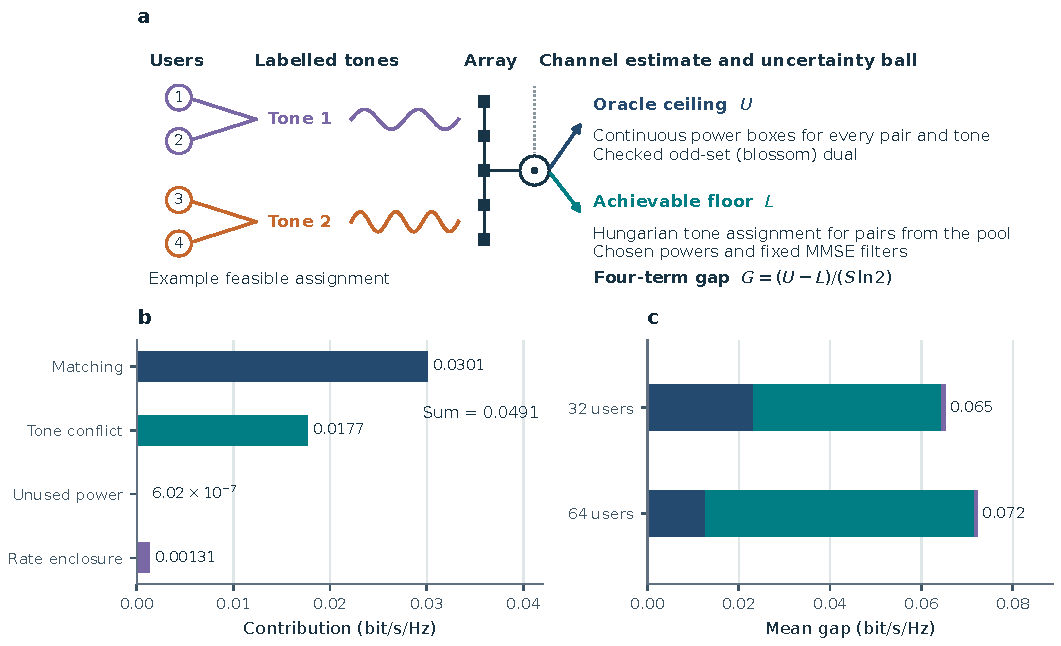
\includegraphics[width=\linewidth]{figures/fig1_architecture.pdf}
\caption{\textbf{A scheduling decision with a rate interval.} \textbf{a}, Users 1 and 2 share tone 1, and users 3 and 4 share tone 2 at the same receive array. Bounds for every pair, tone and power rectangle and a checked matching dual give a ceiling \(U\) for an oracle that can reoptimize its filters. A feasible tone assignment, transmit powers and stored filters give the achievable floor \(L\). \textbf{b}, The four contributions to the gap on the first 32-user CDL-A test topology at 10 dB. \textbf{c}, Mean contributions on 512 test topologies at each size, in the order and colours of \textbf{b}. Component means add to the mean gap.}\label{fig:arch}
\end{figure}
\clearpage\begin{figure}[p]\centering
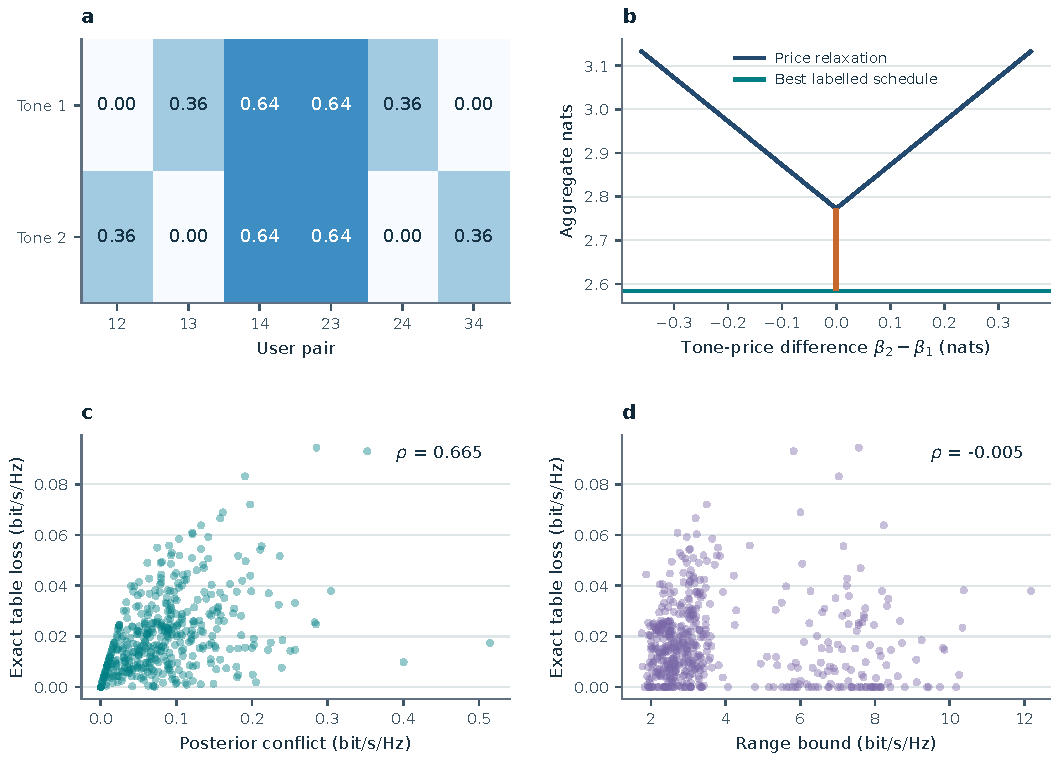
\includegraphics[width=\linewidth]{figures/fig2_conflict.pdf}
\caption{\textbf{Preferred tones and the cost of losing their labels.} \textbf{a}, Squared normalized inner products for the six possible pairs on the two tones of the four-user example. A zero indicates orthogonal channels. \textbf{b}, Exact price relaxation near equal prices and optimal labelled rate of those four users. The marked separation is \(2\ln(100/91)\) aggregate nats. \textbf{c,d}, Exact labelled-table loss versus posterior conflict (\textbf{c}) and the all-edge range bound (\textbf{d}). Each point is one 16-user channel realization at 10 dB, with 128 from each of four simulated profiles. The two horizontal axes have different scales. Coefficients are Spearman rank correlations.}\label{fig:con}
\end{figure}
\clearpage\begin{figure}[p]\centering
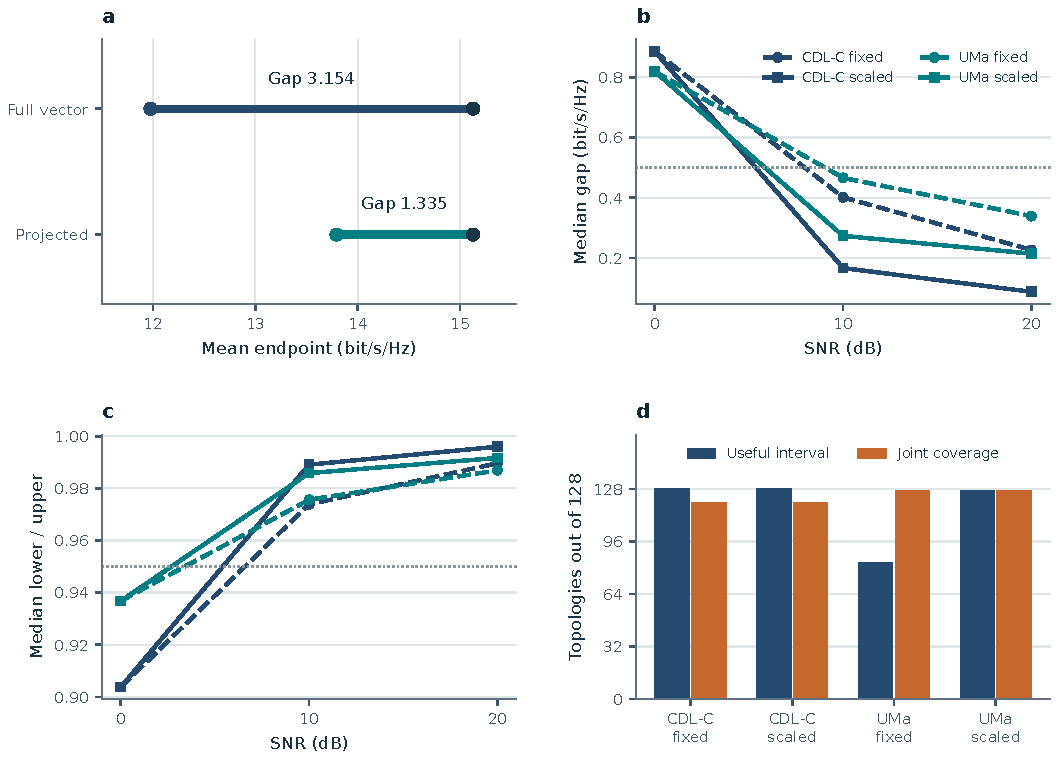
\includegraphics[width=\linewidth]{figures/fig3_uncertainty.pdf}
\caption{\textbf{The deployed receiver and the oracle need different information about channel error.} \textbf{a}, Expected endpoints obtained by integrating finite-sample order statistics. Both rows have the same upper endpoint. \textbf{b,c}, Median projected gap and certified rate retention at 32 users on CDL-C and four-site UMa, with fixed or SNR-scaled pilot energy (128 held-out topologies per family at each SNR). Dotted lines mark 0.50 bit/s/Hz and 0.95 retention. \textbf{d}, Counts at 10 dB meeting all four utility conditions and counts for which both calibrated error events held.}\label{fig:unc}
\end{figure}
\clearpage\begin{figure}[p]\centering
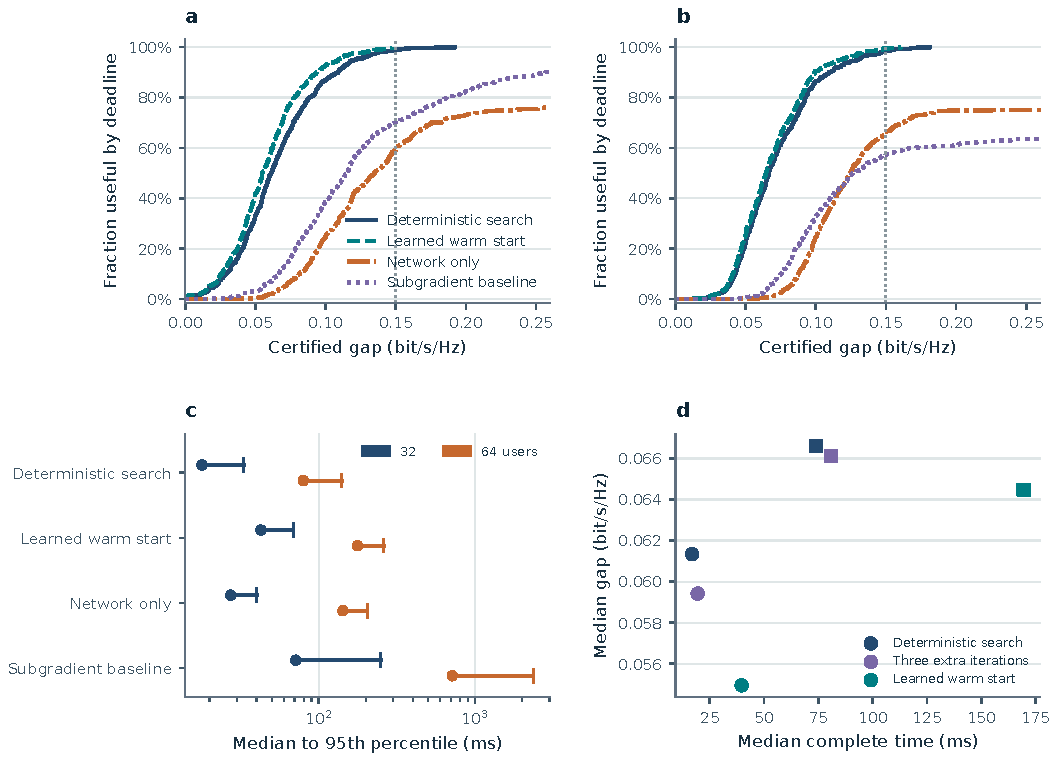
\includegraphics[width=\linewidth]{figures/fig4_scaling.pdf}
\caption{\textbf{Certified gaps and decision times across price-search strategies.} \textbf{a,b}, At each gap on the horizontal axis, the curves show the fraction of all 512 native topologies at 10 dB for which the scheduler achieved that gap or smaller within the deadline. Each topology contributes its largest gap and median time over three calls. The vertical line marks 0.15 bit/s/Hz. \textbf{c}, Filled points mark the median across topology-median wall times. Vertical caps mark the 95th percentile across all timed calls on a logarithmic time axis. \textbf{d}, Median gaps and times in the paired iteration- and time-budget reruns. Filled markers show the iteration run; open markers show the time-budget run. Circles and squares indicate 32 and 64 users. The time-budget control uses 38 and 63 iterations at 32 and 64 users, respectively, versus 10 and 9 for learning. These exploratory timings are separate from panels a--c.}\label{fig:scale}
\end{figure}
\clearpage\begin{figure}[p]\centering
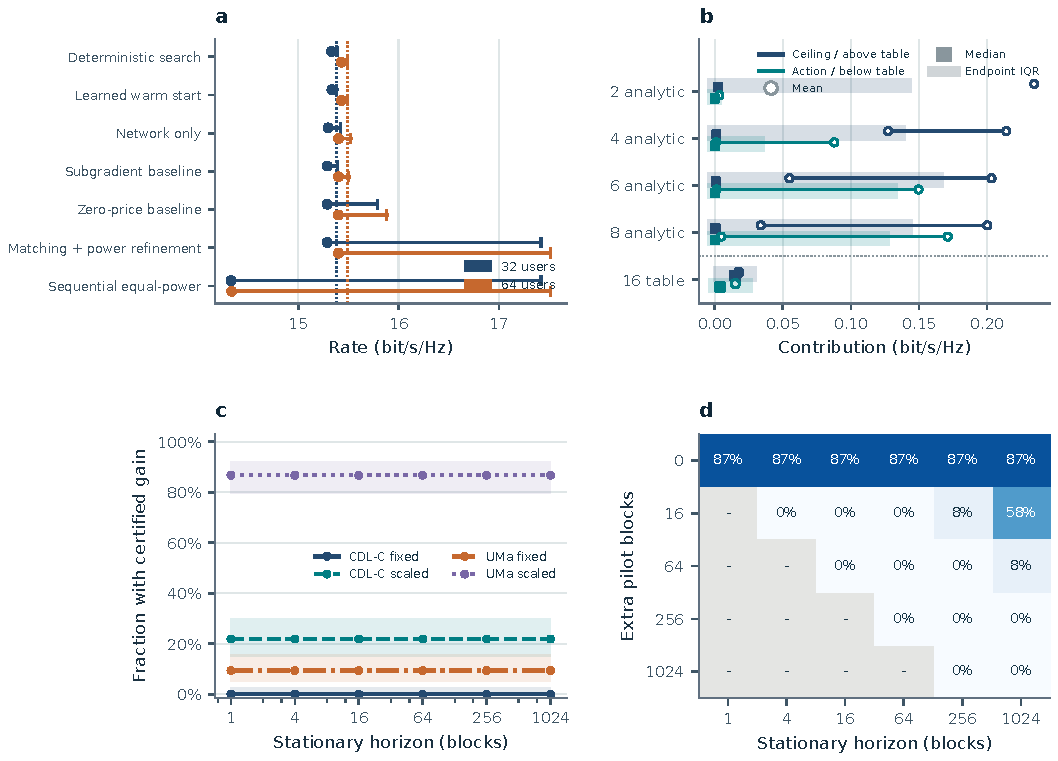
\includegraphics[width=\linewidth]{figures/fig5_phase.pdf}
\caption{\textbf{Achieved rates, remaining optimality uncertainty and the cost of pilots.} \textbf{a}, Median certified lower rates and each method's median upper endpoint on 512 native topologies per size; the best upper endpoint is selected separately within each topology. \textbf{b}, Physical slack/loss brackets on analytic channels through eight users: open circles mark mean endpoints, squares median endpoints, and pale bars span the lower endpoint's first quartile to the upper endpoint's third quartile. The separated 16-user native row instead compares with the exact upper-table optimum. Each row uses 512 topologies; Supplementary Table~8 gives both endpoint IQRs. \textbf{c}, Fractions of 128 independent simulated topologies per arm with a certified positive net gain, with exact two-sided 95\% binomial intervals. \textbf{d}, Scaled UMa fractions when additional pilots are charged over a stationary horizon; grey cells are unaffordable.}\label{fig:phase}
\end{figure}
\clearpage\begin{figure}[p]\centering
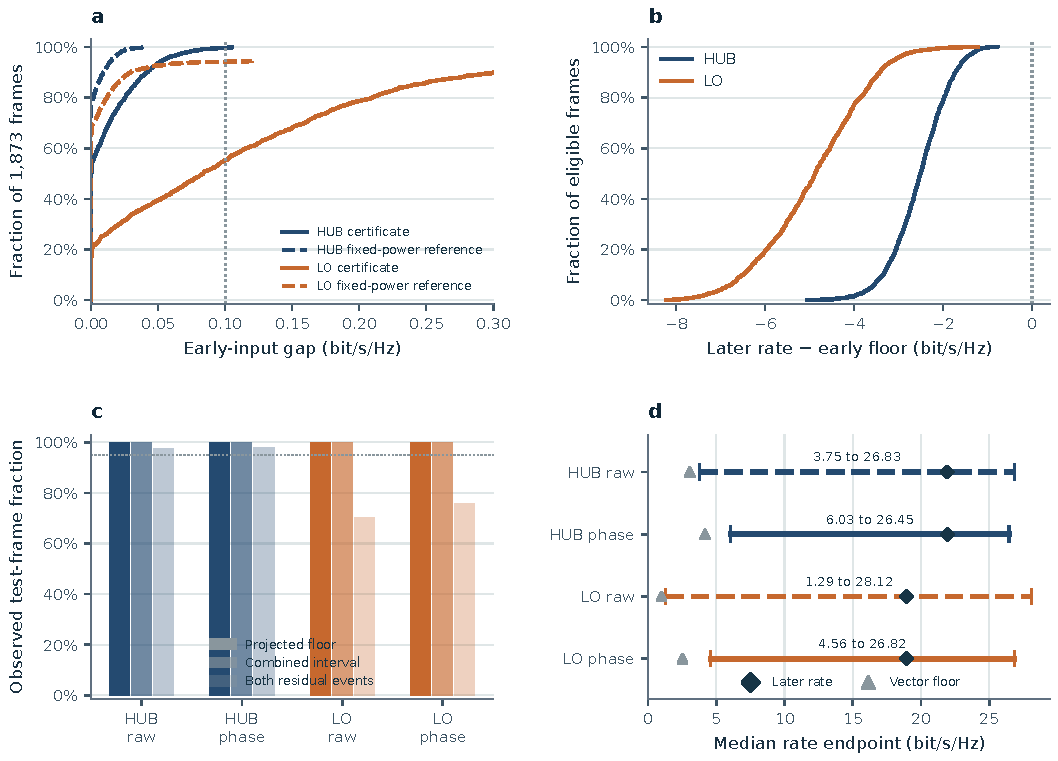
\includegraphics[width=\linewidth]{figures/fig6_hardware.pdf}
\caption{\textbf{Early-input certificates and chronological calibration on recorded pilots.} \textbf{a}, Solid curves show the fraction of all 1,873 post-prefix frames with an early-input certificate below the indicated gap within 250 ms. Dashed curves show the early ceiling minus the exhaustive 90-schedule fixed-equal-power optimum, without a timing cutoff. All curves retain abstentions in the denominator; gaps above 0.30 lie outside the displayed range. \textbf{b}, Later-LTS rate of the stored action minus its uncalibrated early floor on 1,870 HUB and 1,769 LO eligible frames; the two LTS windows begin 16~$\mu$s apart. \textbf{c}, Test-frame coverage under raw and phase-invariant scores: projected floor, combined interval $[\max(L_P,L_F),U_F]$ and both residual events. The dotted line marks 95\%. \textbf{d}, Median projected floors and vector ceilings, with diamonds for later rates and triangles for vector floors. Phase-invariant intervals use projection-magnitude and phase-aligned vector residuals. HUB and LO have 1,614 and 1,513 test frames; Supplementary Table~13 gives paired widths and floor fractions.}\label{fig:hw}
\end{figure}
\end{document}
